%\documentstyle[epsf,twocolumn]{jarticle}       %LaTeX2.09仕様
\documentclass[twocolumn]{jarticle}     %pLaTeX2e仕様

%\usepackage[backend=bibtex, style=numeric]{biblatex}
%\addbibresource{sankou.bib}
%%%%%%%%%%%%%%%%%%%%%%%%%%%%%%%%%%%%%%%%%%%%%%%%%%%%%%%%%%%%%%
%%
%%  基本 バージョン
%%
%%%%%%%%%%%%%%%%%%%%%%%%%%%%%%%%%%%%%%%%%%%%%%%%%%%%%%%%%%%%%%%%
\setlength{\topmargin}{-45pt}
%\setlength{\oddsidemargin}{0cm}
\setlength{\oddsidemargin}{-7.5mm}
%\setlength{\evensidemargin}{0cm}
\setlength{\textheight}{24.1cm}
%setlength{\textheight}{25cm}
\setlength{\textwidth}{17.4cm}
%\setlength{\textwidth}{172mm}
\setlength{\columnsep}{11mm}

\setlength{\intextsep}{8pt}
\setlength{\textfloatsep}{8pt}
\setlength{\floatsep}{1pt}

\kanjiskip=.07zw plus.5pt minus.5pt



%【節がかわるごとに(1.1)(1.2) …(2.1)(2.2)と数式番号をつけるとき】
%\makeatletter
%\renewcommand{\theequation}{%
%\thesection.\arabic{equation}} %\@addtoreset{equation}{section}
%\makeatother

%\renewcommand{\arraystretch}{0.95} 行間の設定

\usepackage[dvipdfmx]{graphicx}   %pLaTeX2e仕様(\documentstyle ->\documentclass)
\usepackage[dvipdfmx]{color}
\usepackage{scalefnt}
\usepackage{bm}
\usepackage{here}
\usepackage{url}
\usepackage{amsmath}
\usepackage{amsfonts}
\usepackage[subrefformat=parens]{subcaption}
\captionsetup{compatibility=false}
%%%%%%%%%%%%%%%%%%%%%%%%%%%%%%%%%%%%%%%%%%%%%%%%%%%%%%%%
\usepackage{comment}
\usepackage{subcaption}
\usepackage{multirow}
\usepackage{nidanfloat}
%\usepackage[table,xcdraw]{xcolor}
\usepackage[dvipdfmx]{hyperref}

\usepackage[normalem]{ulem}
\useunder{\uline}{\ul}{}

\begin{document}

\twocolumn[
\noindent
\hspace{1em}

令和2年6月24日(水) ゼミ資料
\hfill
\ \ B4 高山 裕成

\vspace{2mm}
\hrule
\begin{center}
{\Large  進捗報告}
\end{center}
\hrule
\vspace{3mm}
]

% \footnotesize
\section{進捗}

\begin{itemize}
  \item 連続 n 文を入力とし, 正例ラベルを喜楽としたときの 2 クラス感情推定
\end{itemize}

\section{実験設定}
図\ref{fig:net} にネットワークの概略図を示す. ${s_i}$ はそれぞれ連続する n 文のセリフを BERT の id 列に変換したものである. また, 組み合わせとしては同一の 4 コマに属し, かつ連続しているものを扱う. 各 4 コマの序盤に現れるセリフには参照できる過去のセリフが無いため, 便宜上のセリフ $[$pad$]$ を置くことで対処した. 末尾のセリフ以外はオリジナルのセリフのみから抽出することで, データ数を合わせている.

よって, 単語 id 列長を $w$ とすると入力次元は $(batch \times n \times w)$ となる. このままでは BERT の入力次元に対応していないので, まず $(n \times batch \times w)$ へと軸を入れ替え, これを 1 次元目について各要素に分解し, これら n 個の 次元数 $(batch \times w)$ のベクトルをそれぞれ BERT への入力とし, BERT の出力から [CLS] トークンに相当するベクトルのみを抜き取り, 先と逆の手順を踏むことで次元数 $(batch \times n \times 768)$ のテンソルを得ることができる. これを識別器 Bi LSTM, Self-Attention への入力とすることで末尾のセリフの感情推定を行う.

BERT は事前学習済モデル\footnote{http://nlp.ist.i.kyoto-u.ac.jp}を用い, 最終層のみをチューニングする. その他実験設定などは, 前回までと同様 1 文のみを入力とする実験と同じである. 識別器のパラメータは図\ref{tab:self_net} に示す.

今週は $n = 3$ と $n = 5$ の場合について実験を行った.

\begin{figure}[!hb]
  \begin{center}
    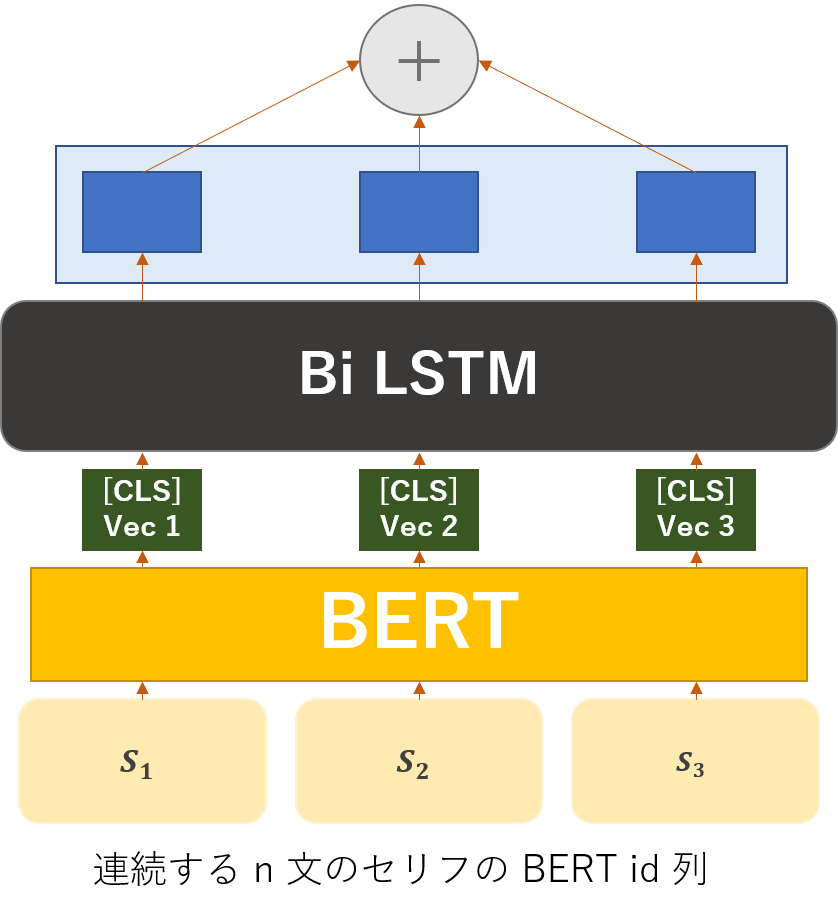
\includegraphics[scale=0.3]{net.png}
    \caption{seq net} %タイトルをつける
    \label{fig:net} %ラベルをつけ図の参照を可能にする
  \end{center}
\end{figure}

\begin{table}[tbh]
\begin{center}
\caption{network parameters}
\begin{tabular}{|c|c|}
\hline
parameter & value \\ \hline
lstm\_in & 300   \\
lstm\_hidden    & 128    \\
self\_atten\_in & $128 \times 2$     \\
atten\_num\_layers & 3     \\ \hline
\end{tabular}
\label{tab:self_net}
\end{center}
\end{table}

\section{実験結果}
表\ref{tab:result} に実験結果を載せる. 表\ref{tab:result} より B3 実験の時と同様で n を大きくすることで Accuracy が下がり, 正例の Recall と F1 値が上がる傾向が見られると予想できる. (不均衡データでも過剰に正例だと判定するようになる.)


\begin{table*}[thb]
\begin{center}
\caption{result}
\scalebox{0.6}{
\begin{tabular}{llcllcllcllcllcll|cll}
\hline
\multicolumn{2}{c}{\multirow{2}{*}{seq len}} & \multicolumn{3}{c}{ギャグ} & \multicolumn{3}{c}{少女漫画} & \multicolumn{3}{c}{少年漫画} & \multicolumn{3}{c}{青年漫画} & \multicolumn{3}{c|}{萌え系} & \multicolumn{3}{c|}{5タッチ平均} \\
\multicolumn{2}{c}{} & Acc & \multicolumn{1}{c}{Recall} & \multicolumn{1}{c}{F1} & Acc & \multicolumn{1}{c}{Recall} & \multicolumn{1}{c}{F1} & Acc & \multicolumn{1}{c}{Recall} & \multicolumn{1}{c}{F1} & Acc & \multicolumn{1}{c}{Recall} & \multicolumn{1}{c}{F1} & Acc & \multicolumn{1}{c}{Recall} & \multicolumn{1}{c|}{F1} & Acc & \multicolumn{1}{c}{Recall} & \multicolumn{1}{c}{F1} \\ \hline
\multicolumn{2}{l}{3} & \multicolumn{1}{l}{\textbf{0.773}} & 0.000 & 0.000 & \multicolumn{1}{l}{\textbf{0.627}} & 0.526 & \textbf{0.615} & \multicolumn{1}{l}{\textbf{0.766}} & 0.000 & 0.000 & \multicolumn{1}{l}{\textbf{0.800}} & \textbf{0.286} & \textbf{0.381} & \multicolumn{1}{l}{\textbf{0.625}} & \textbf{0.409} & \textbf{0.429} & \multicolumn{1}{l}{\textbf{0.718}} & 0.244 & 0.285 \\
\multicolumn{2}{l}{5} & \multicolumn{1}{l}{0.591} & \textbf{0.600} & \textbf{0.308} & \multicolumn{1}{l}{0.552} & \textbf{0.553} & 0.583 & \multicolumn{1}{l}{0.578} & \textbf{0.333} & \textbf{0.229} & \multicolumn{1}{l}{0.585} & 0.214 & 0.182 & \multicolumn{1}{l}{0.547} & \textbf{0.409} & 0.383 & \multicolumn{1}{l}{0.571} & \textbf{0.422} & \textbf{0.337} \\ \hline
\multicolumn{2}{l}{ベースライン} & 0.85 & \multicolumn{1}{c}{0} & \multicolumn{1}{c}{0} & 0.43 & \multicolumn{1}{c}{0} & \multicolumn{1}{c}{0} & 0.81 & \multicolumn{1}{c}{0} & \multicolumn{1}{c}{0} & 0.78 & \multicolumn{1}{c}{0} & \multicolumn{1}{c}{0} & 0.66 & \multicolumn{1}{c}{0} & \multicolumn{1}{c|}{0} & 0.71 & \multicolumn{1}{c}{0} & \multicolumn{1}{c}{0}
\end{tabular}
\label{tab:result}
}
\end{center}
\end{table*}

\section{今後の研究の方向性?}
\begin{itemize}
  \item 4 コマストーリーデータセットで訓練・テストでは精度に期待できない
  \item 整備された他の日本語の極性評価データセットを用いて BERT の事前学習モデルを fine tuning し, 4 コマ漫画の感情推定問題に転移させる?
  \item 仕様によっては感情ラベルの貼り直し, または人手によるラベル付けが必要になる
  \item manga109 のセリフのデータも用いれば半教師あり学習も可能か
\end{itemize}



\section{今後の実験予定}
\begin{itemize}
  \item 前期発表資料作り
  \item 連続 n 文を入力とする実験 続き
  \item コマの画像のベクトルも考慮した感情推定
\end{itemize}

\bibliographystyle{unsrt}
\bibliography{sankou}


\end{document}
